% HARE -- DAC submission draft.
% Tables under tables/ are generated by gen_tables.py from
% docs/proposals/data/crypto_measurements.csv and the archived Quartus
% reports; regenerate rather than editing them.
\documentclass[conference]{IEEEtran}
\usepackage[T1]{fontenc}
\usepackage{booktabs}
\usepackage{tikz}
\usepackage{balance}

\newcommand{\cB}{c/B}
\newcommand{\ie}{i.e.,\ }
\newcommand{\eg}{e.g.,\ }

\begin{document}

\title{HARE: High-Throughput Authenticated Encryption\\
for RISC-V GPGPUs via an ISE}

\author{\IEEEauthorblockN{Anonymous authors}
\IEEEauthorblockA{Paper under double-blind review}}

\maketitle

\begin{abstract}
Authenticated encryption (AEAD) now guards every path data takes between
devices, and GPGPUs increasingly produce and consume that data---yet the GPU
is the one place the AEAD itself cannot run cheaply. Software AES-GCM costs
70.9 cycles per byte on our platform, and fixed-function engines freeze the
algorithm at tape-out and sit outside the programming model.
This paper presents HARE, a systematic study of the instruction-set-extension
design space for AEAD on SIMT GPGPUs. We organize the space into four tiers
by where the cipher's block state lives---S0 software, S1 lane-local
instructions, S2 stateful engines, S3 subgroup-cooperative instructions---and
implement AES-GCM and ChaCha20-Poly1305 at every tier in the RTL of an
open-source RISC-V GPGPU. Measurement yields three results. First, the two
algorithms harvest at different tiers: lane-local instructions, the SIMT
analogue of the ratified scalar cryptography extensions, deliver
$18.4\times$ for AES-GCM but only $1.67\times$ for ChaCha20-Poly1305.
Second, subgroup-cooperative instructions are the best tier for both
algorithms once the subgroup spans the cipher's block state: four lanes for
AES's 128-bit state ($4.15\times$ over lane-local), sixteen for ChaCha's
512-bit state ($4.97\times$, where a four-lane form returns $1.25\times$).
Third, state \emph{inside one instruction's execution} occupies an interior
optimum between stateless instructions, which bottleneck on issue bandwidth,
and architectural context, which costs $2.7\times$ the area plus key-lifetime
semantics. All designs close timing at 200\,MHz on a Stratix~10 FPGA; the
recommended ChaCha pair adds 2.8\% to the core it extends. End to end, HARE
reaches $76\times$ (AES-GCM) and $8.3\times$ (ChaCha20-Poly1305) over
software.
\end{abstract}

\section{Introduction}\label{sec:intro}

Data in flight is now encrypted by default, and almost all of it under one of
two authenticated ciphers: AES-GCM~\cite{sp800-38d,mcgrew2004gcm} and
ChaCha20-Poly1305~\cite{rfc8439} carry TLS~1.3, QUIC, disk and object
storage, and---most recently---the secured CPU--GPU and GPU--GPU links of
confidential accelerators~\cite{nvidia-h100-cc,lee2025gputee}. Over the same
decade, GPGPUs have become the place where this data is produced and
consumed. The two trends meet badly: the machine that touches the data is
the one machine that cannot afford to encrypt it.

A SIMT core today has two options. It can run the AEAD in software over the
base ISA: on the open-source Vortex GPGPU~\cite{tine2021vortex} we measure
70.9 cycles per byte (\cB) for AES-GCM---and the fast software AES it uses,
T-tables, is also the canonical cache-timing victim. Or the system can bolt
on a fixed-function engine: fast, but frozen at tape-out, reachable only by
DMA round-trip, and closed to every algorithm chosen after silicon. CPUs
resolved this same tension a decade ago with ISA extensions---AES-NI on
x86~\cite{gueron2010aesni}, and for RISC-V the ratified scalar
(Zkn/Zbc)~\cite{riscv-scalar-crypto} and vector (Zvk)~\cite{riscv-vector-crypto}
cryptography extensions. Inside a SIMT pipeline, the corresponding design
space is essentially unexplored.

Exploring it produces two surprises. The obvious first step is to port the
scalar extensions into every lane. This helps unevenly: it buys AES-GCM
$18.35\times$, because it deletes the table lookups, but ChaCha20-Poly1305
only $1.67\times$, because ARX rounds were never table-bound---the
correct-by-construction port of the ratified extensions leaves the second
cipher almost untouched. The obvious second step is a stateful engine: write
the key once into hardware context, then stream blocks through it. It
works---$2.23\times$ and $3.78\times$ over the lane-local tier---but it is
the most expensive point in the space (+115{,}936 ALMs on a 183{,}971-ALM
core for AES-GCM), and it plants per-(warp,\,lane) key material in the
pipeline, with the zeroize-on-ownership-change and save-or-destroy-on-%
preemption semantics that resident secrets drag behind them. It is also,
on both algorithms, not the fastest tier.

HARE's answer is a third structure and two design rules. In the
\emph{subgroup-cooperative} tier, the cipher's block state never leaves the
register file: it lies spread one 32-bit word per lane across an aligned
group of lanes, and a single instruction reads that group's registers with
fixed routing and advances an entire round---or absorbs an entire block.
No architectural state exists anywhere. The first rule is that the subgroup
must span the cipher's block state: AES's 128-bit state is four lanes wide
and a four-lane form returns $4.15\times$; ChaCha's 512-bit state is sixteen
lanes wide, and the same four-lane structure that serves AES returns
$1.25\times$ where a sixteen-lane form returns $4.97\times$. The second rule
concerns the state a multi-cycle instruction holds \emph{while it executes}:
none at all bottlenecks on issue bandwidth ($2.19\times$ slower), and full
architectural context pays $2.7\times$ the area and the lifetime semantics;
1{,}154 bits of instruction-internal working registers---the interior
point---beats both ends.

This paper contributes:
\begin{itemize}
\item a design-space taxonomy (S0--S3) for AEAD ISEs in SIMT pipelines,
  organized by where the cipher's block state lives, with every tier
  implemented for two AEADs in the RTL of an open-source RISC-V GPGPU and
  verified against NIST and RFC test vectors in two independent models;
\item the measurement that the two AEADs harvest at different tiers, and
  that the subgroup-cooperative tier is the best for both---$4.15\times$ and
  $4.97\times$ over lane-local, $76\times$ and $8.3\times$ over software;
\item the width rule, with the $1.25\times{\to}4.97\times$ inversion that
  follows from matching the subgroup to the block state; and
\item the state-placement result: an interior optimum between stateless
  and stateful designs, with the issue-bandwidth mechanism that explains
  it---plus the engineering result that the entire extension fits standard
  two-read-one-write operand delivery.
\end{itemize}

All measurements derive from a committed, per-run measurement record and
archived place-and-route reports; every design closes timing at 200\,MHz on
a Stratix~10 FPGA.

\section{Background}\label{sec:background}

\subsection{SIMT execution and subgroups}
A SIMT core executes \emph{warps}; each warp issues one instruction over
$k$ \emph{lanes} (here $k{=}16$), and each lane owns a private scalar
register file. A \emph{subgroup} is an aligned group of lanes within one
warp (lanes $4q..4q{+}3$ for width four; all sixteen for width sixteen).
Vortex~\cite{tine2021vortex} is an open-source RISC-V GPGPU with this
organization; our configuration is two cores, four warps per core, sixteen
lanes per warp, RV32IM.

\subsection{Two AEADs, by state size}
AES-GCM encrypts 16-byte blocks through 10--14 rounds over a
\textbf{128-bit} state and authenticates with GHASH, a multiply in
GF($2^{128}$)~\cite{sp800-38d}. ChaCha20 keeps a \textbf{512-bit} state of
sixteen 32-bit words; a double round applies eight add-xor-rotate (ARX)
quarter-round lines across columns and then diagonals~\cite{bernstein2008chacha}.
Poly1305 absorbs 16-byte blocks into a 130-bit accumulator held as five
26-bit limbs~\cite{bernstein2005poly}. Two numbers in this paragraph do all
the work in Section~\ref{sec:eval}: $128 = 4\times$ a 32-bit lane, and
$512 = 16\times$.

\section{The design space: where the state lives}\label{sec:space}

We organize AEAD ISEs for SIMT machines into four tiers
(Fig.~\ref{fig:tiers}), distinguished by a single question: \emph{where does
the cipher's block state live, and what may one instruction read?}

\textbf{S0 --- software.} State lives in per-lane registers and memory; an
instruction reads two registers of one lane. Every state move and table
lookup is explicit.

\textbf{S1 --- lane-local.} Same state residence; an instruction now
performs a cipher \emph{step} (a T-less AES round step, a carry-less
multiply, an xor-rotate, a 26-bit multiply-accumulate) but still sees only
one lane's two operands. This is the SIMT port of the ratified scalar
extensions~\cite{riscv-scalar-crypto}.

\textbf{S2 --- stateful engine.} State moves out of the register file into
unit-private \emph{architectural context}, addressed by (warp,\,lane).
Context-write instructions load key and nonce once; per-block instructions
then reference the context implicitly, so the instruction stream shrinks to
data in, data out. The context survives between instructions---which is
precisely what gives this tier its cost: storage for every (warp,\,lane),
and a lifetime: who owns it, when it is valid, and when it must be zeroized.

\textbf{S3 --- subgroup-cooperative.} State returns to the register file,
but spread one word per lane across an aligned subgroup; a single
instruction reads the subgroup's operand vector with \emph{fixed} lane
routing (no crossbar) and writes one result per lane. Nothing survives the
instruction. S2 changes where state lives; S3 changes only \emph{who may
read it}.

Three properties frame everything that follows. All instructions of tiers
S1--S3 have fixed, data-independent latency and no data-dependent memory
access, so every hardware tier is constant-time by construction---unlike the
T-table software they replace. Subgroup instructions require their subgroup
fully converged (the mask must cover all lanes of the group; both our models
assert it). And only S2 creates resident secrets: S1 and S3 leave nothing in
the pipeline for a context switch to leak.

\begin{figure}[t]
\centering
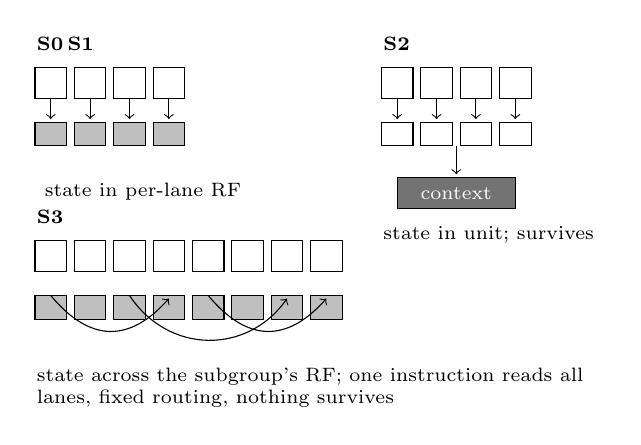
\begin{tikzpicture}[font=\scriptsize, x=1mm, y=1mm]
\foreach \px/\name/\mode in {0/S0\,S1/rf, 44/S2/ctx} {
  \begin{scope}[shift={(\px,0)}]
    \foreach \i in {0,1,2,3}
      \draw (\i*5,8) rectangle +(4,4);
    \node[anchor=west] at (-1,15) {\textbf{\name}};
    \ifx\mode\relax\fi
  \end{scope}
}
% S0/S1: state in per-lane RF
\foreach \i in {0,1,2,3} \fill[black!25] (\i*5,2) rectangle +(4,3);
\draw (0,2) node[anchor=north west, yshift=-3.5mm] {state in per-lane RF};
\foreach \i in {0,1,2,3} \draw (\i*5,2) rectangle +(4,3);
\foreach \i in {0,1,2,3} \draw[->] (\i*5+2,8) -- (\i*5+2,5.4);
% S2: state in unit context
\begin{scope}[shift={(44,0)}]
  \foreach \i in {0,1,2,3} \draw (\i*5,2) rectangle +(4,3);
  \fill[black!55] (2,-6) rectangle +(15,4);
  \draw (2,-6) rectangle +(15,4);
  \node[white] at (9.5,-4) {context};
  \foreach \i in {0,1,2,3} \draw[->] (\i*5+2,8) -- (\i*5+2,5.4);
  \draw[->] (9.5,2) -- (9.5,-1.6);
  \node[anchor=north west] at (-1,-7) {state in unit; survives};
\end{scope}
% S3 panel below, spanning
\begin{scope}[shift={(0,-22)}]
  \node[anchor=west] at (-1,15) {\textbf{S3}};
  \foreach \i in {0,...,7} \draw (\i*5,8) rectangle +(4,4);
  \foreach \i in {0,...,7} \fill[black!25] (\i*5,2) rectangle +(4,3);
  \foreach \i in {0,...,7} \draw (\i*5,2) rectangle +(4,3);
  \draw[->] (2,5) .. controls (7,-1) and (12,-1) .. (17,4.6);
  \draw[->] (22,5) .. controls (27,-1) and (32,-1) .. (37,4.6);
  \draw[->] (12,5) .. controls (17,-2.5) and (27,-2.5) .. (32,4.6);
  \node[anchor=north west, text width=72mm, align=left] at (-1,-3)
    {state across the subgroup's RF; one instruction reads all lanes,
     fixed routing, nothing survives};
\end{scope}
\end{tikzpicture}
\caption{The four tiers, by where the block state lives. S2 moves state into
hidden context; S3 leaves it architectural in the register file and lets one
instruction read it across lanes.}
\label{fig:tiers}
\end{figure}

\section{The HARE instructions}\label{sec:ise}

Table~\ref{tab:isa} lists the extension. Every instruction is R-type with at
most two source reads and one write; no tier requires a third register-file
read port or any operand path the base machine lacks.

\begin{table}[t]
\centering
\caption{The HARE ISEs. All are 2R1W R-type; subgroup forms read their
operands across an aligned quad (\texttt{.sg4}) or sixteen lanes
(\texttt{.sg16}).}
\label{tab:isa}
\scriptsize
\setlength{\tabcolsep}{2.5pt}
\begin{tabular}{@{}lll@{}}
\toprule
Tier & AES-GCM & ChaCha20-Poly1305 \\
\midrule
S1 & \texttt{aes32esi/esmi} round steps & \texttt{chacha32.xr} xor-rotate \\
   & \texttt{clmul/h}, \texttt{ghred32/h} & \texttt{poly26.mac} \\
\addlinespace
S2 & \texttt{aes.cwr/begin/rndm/rndf/crd} & \texttt{cha.cwr/dr/crd} \\
   & \texttt{ghash.cwr/init/block/crd} & \\
\addlinespace
S3 & \texttt{aesrm.sg4} full round & \texttt{chacha.dr.sg16} double round \\
   & \texttt{ghmul.sg4} GF mul & \texttt{poly4.step.sg16} 64-B absorb \\
\bottomrule
\end{tabular}
\end{table}

\subsection{S1: the scalar extensions, in every lane}
The AES path follows the ratified 32-bit constructions: \texttt{aes32esi}
and \texttt{aes32esmi} compute one table-free round step per lane, and GHASH
is built from carry-less multiplies (\texttt{clmul/clmulh}) plus two
reduction helpers (\texttt{ghred32/ghred32h}). ChaCha gets a fused
xor-rotate and Poly1305 a 26-bit limb multiply-accumulate. These
instructions define the tier every later number is normalized to.

\subsection{S2: stateful engines}
Context-write instructions (\texttt{.cwr}) load key, nonce and counter into
unit-private storage; streaming instructions then advance whole blocks.
The ChaCha context is 896 bits per (warp,\,lane)---512 state, 256 key, 96
nonce, 32 counter---which at four warps and sixteen lanes is 57{,}344 bits
per core, and the register cost of an S2 engine is predictable from its
context definition to within 2.4\%. The engines are fixed-latency and
per-lane; their cost is evaluated in Section~\ref{sec:eval}.

\subsection{S3: subgroup-cooperative instructions}
For AES-GCM the subgroup is an aligned quad: lane $i$ holds column $i$ of
the 128-bit state, \texttt{aesrm.sg4} performs a complete round (the
ShiftRows lane exchange is fixed wiring), and \texttt{ghmul.sg4} a
GF($2^{128}$) multiply. For ChaCha the subgroup is sixteen lanes: lane $i$
holds word $i$ of the 512-bit state and \texttt{chacha.dr.sg16} advances one
full double round per instruction---ten instructions per block. It executes
as a fixed ten-cycle sequence over 1{,}154 bits of working registers,
owner-locked while in flight; nothing survives the instruction.
\texttt{poly4.step.sg16} absorbs a whole 64-byte ChaCha block---four
Poly1305 blocks---in one instruction: the accumulator $h$ travels in lanes
0--4, the key $r$ in lanes 5--9 of the \emph{same} source register, and the
result returns $h'$ with $r$ untouched, so the output feeds the next
absorb directly. The $r^2,r^3,r^4$ schedule that block-parallel software
Poly1305 must hold in registers (we measure it at 36\% of kernel cycles)
exists only inside the unit, and never becomes architectural.

\subsection{Encoding}
Packing $h$ and $r$ into one operand is what keeps the tier 2R1W: the first
version of \texttt{poly4.step.sg16} read them from two registers and needed
an R4-type third read port. Ten of sixteen lanes carry both values with six
to spare; the repack costs +218 ALMs and 17 instructions per message
(${<}2\%$ of cycles), and returns a seven-bit funct7 where R4 offers two
bits. One caution generalizes: our four-bit sub-opcode space filled
completely---the sixteen-lane double round shares a slot with the S2 engine
op, and the build system refuses the combination---so an extension of this
size should budget opcode space as deliberately as it budgets area.

\section{Methodology}\label{sec:method}

All cycle counts come from Verilator simulation of the synthesized RTL
configuration (two cores $\times$ four warps $\times$ sixteen lanes) with a
DDR4 model; instruction counts from an independent functional simulator that
agrees with the RTL to the instruction. Both models pass the NIST GCM and
RFC~8439 test vectors for every implementation at every tier. Simulation is
deterministic---repeated runs are byte-identical---so every difference we
report is a design difference, not noise. Per-byte figures are two-point
marginal fits between 64\,KiB and 128\,KiB total payloads (and 4--16\,KiB
for cache-resident figures), which cancels per-message setup;
fits never mix builds. Area and timing come from Quartus place-and-route for
a DE10-Pro (Stratix~10 1SG280HU1F50E1VG) with a 200\,MHz GPU clock; we
report a build only if its GPU clock domain closes in every one of the 30
timing-model/corner entries. The per-run measurement record (444 rows), the
RTL, and the place-and-route reports accompany the paper.

\section{Evaluation}\label{sec:eval}

\begin{table}[t]
\centering
\caption{The tier ladder. Memory-bound marginal cycles and instructions per
byte; speedups against each algorithm's own S0 and S1. $\Delta$ALM is the
whole build against the crypto-free core (183{,}971 ALMs); each build
includes its lane-local parent units.}
\label{tab:tiers}
\scriptsize
\setlength{\tabcolsep}{3.5pt}
%% generated by gen_tables.py -- do not edit
\begin{tabular}{@{}llrrrrr@{}}
\toprule
 & Tier & c/B & instr/B & $\times$S0 & $\times$S1 & $\Delta$ALM \\
\midrule
AES-GCM & S0 software & 70.865 & 18.566 & 1.00 & 0.05 & 0 \\
 & S1 lane-local & 3.862 & 1.578 & 18.35 & 1.00 & +24,542 \\
 & S2 stateful engine & 1.733 & 0.262 & 40.89 & 2.23 & +115,936 \\
 & \textbf{S3 subgroup\,/\,4} & \textbf{0.931} & 0.703 & \textbf{76.08} & \textbf{4.15} & +76,967 \\
\midrule
ChaCha-Poly & S0 software & 12.026 & 1.922 & 1.00 & 0.60 & 0 \\
 & S1 lane-local & 7.197 & 1.180 & 1.67 & 1.00 & +33,412 \\
 & S2 stateful engine & 1.903 & 0.451 & 6.32 & 3.78 & +105,382 \\
 & S3 subgroup\,/\,4 & 5.755 & 1.414 & 2.09 & 1.25 & +35,950 \\
 & \textbf{S3 subgroup\,/\,16} & \textbf{1.447} & 0.766 & \textbf{8.31} & \textbf{4.98} & +39,456 \\
\bottomrule
\end{tabular}

\end{table}

\subsection{Different algorithms harvest at different tiers}
Table~\ref{tab:tiers} is the paper's central measurement. Reading the
$\times$S1 column: AES-GCM's big step is S0${\to}$S1 ($18.35\times$)---the
tier that deletes its table lookups---after which the stateful engine adds
$2.23\times$ and the subgroup form $4.15\times$. ChaCha's S1 buys only
$1.67\times$: ARX was never table-bound, and its costs sit in the sheer
count of round operations, which only round-level instructions (S2/S3)
remove. The design consequence: a GPGPU that stops at the ported scalar
extensions has solved AES and left ChaCha almost untouched; one that stops
at stateful engines has paid the most area for neither algorithm's best row.
At both operating points the subgroup tier wins for both AEADs
($5.51\times$/$5.74\times$ over S1 cache-resident). At 200\,MHz the
two-core prototype sustains 215\,MB/s AES-GCM and 138\,MB/s
ChaCha20-Poly1305 at S3---0.86 and 0.55\,Gb/s per core---against
2.8 and 16.6\,MB/s in software.

\subsection{The subgroup must span the block state}
\begin{figure}[t]
\centering
%% generated by gen_tables.py -- do not edit
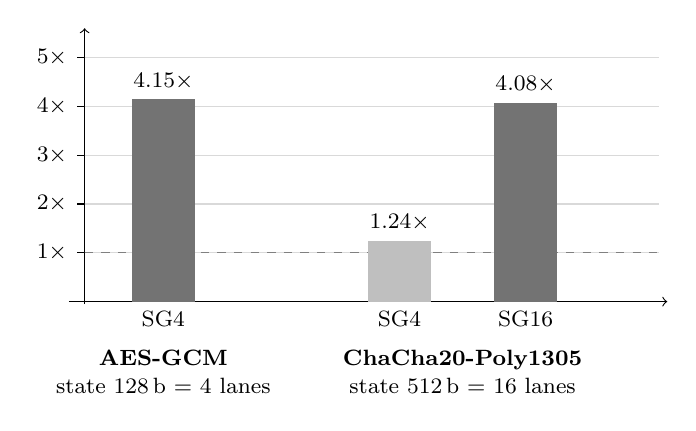
\begin{tikzpicture}[x=1cm,y=0.62cm, font=\footnotesize]
  \draw[->] (-0.2,0) -- (7.4,0) node[below left]{};
  \draw[->] (0,-0.05) -- (0,5.6*1) ;
  \foreach \y in {1,2,3,4,5} {
    \draw (0,\y) -- (-0.1,\y) node[left]{\y$\times$};
    \draw[gray!30] (0,\y) -- (7.3,\y); }
  \draw[dashed,gray] (0,1) -- (7.3,1);
  %% AES-GCM: state 128 b = 4 lanes
  \fill[black!55] (0.6,0) rectangle +(0.8,4.146);
  \node[above] at (1.0,4.146) {4.15$\times$};
  \node[below] at (1.0,0) {SG4};
  \node[below=14pt] at (1.0,0) {\textbf{AES-GCM}};
  \node[below=24pt] at (1.0,0) {state 128\,b $=$ 4 lanes};
  %% ChaCha: state 512 b = 16 lanes
  \fill[black!25] (3.6,0) rectangle +(0.8,1.242);
  \node[above] at (4.0,1.242) {1.24$\times$};
  \node[below] at (4.0,0) {SG4};
  \fill[black!55] (5.2,0) rectangle +(0.8,4.076);
  \node[above] at (5.6,4.076) {4.08$\times$};
  \node[below] at (5.6,0) {SG16};
  \node[below=14pt] at (4.8,0) {\textbf{ChaCha20-Poly1305}};
  \node[below=24pt] at (4.8,0) {state 512\,b $=$ 16 lanes};
\end{tikzpicture}

\caption{Speedup over each algorithm's S1 for subgroup-cooperative forms.
Four lanes is the right width for AES's 128-bit state and the wrong width
for ChaCha's 512-bit state; at sixteen lanes the ChaCha result inverts,
$1.25\times{\to}4.97\times$.}
\label{fig:width}
\end{figure}
Fig.~\ref{fig:width} isolates the width rule. AES-GCM's four-lane form
returns $4.15\times$ because its block state \emph{is} four lanes wide: one
\texttt{aesrm.sg4} holds the whole state, and ShiftRows becomes wiring. The
same four-lane structure applied to ChaCha returns $1.25\times$: a 512-bit
state spans four quads, every quarter-round reads words a \emph{different}
quad holds, and the cross-quad traffic stays in software. Widening the
subgroup to sixteen lanes---the state's own width---turns the diagonal
permutation into fixed routing inside one instruction, and the same
algorithm returns $4.97\times$. Stated as a rule: \emph{a
subgroup-cooperative form pays when the subgroup spans the cipher's block
state; narrower forms leave the state movement in software, and with it most
of the win.} Two ciphers instantiate the rule at $k{=}4$ and $k{=}16$; it is
a property of the block state's extent, not of either cipher.

\subsection{State placement has an interior optimum}
\begin{table}[t]
\centering
\caption{Three placements for the state of the ChaCha round instruction,
same kernel, same machine. The middle wins both axes' trade.}
\label{tab:state}
\scriptsize
\setlength{\tabcolsep}{3pt}
%% generated by gen_tables.py -- do not edit
\begin{tabular}{@{}lrrrr@{}}
\toprule
Where the state lives & bits & instr/64\,B & cyc/64\,B & ALMs \\
\midrule
none (\texttt{chacha.arx.sg16}) & 0 & 142.0 & 203.1 & 217,854 \\
\textbf{working regs (\texttt{chacha.dr.sg16})} & \textbf{1{,}154} & \textbf{49.0} & \textbf{92.6} & \textbf{223,427} \\
architectural context (S2) & 57{,}344 & 28.9 & 121.8 & 289,353 \\
\bottomrule
\end{tabular}

\end{table}
Table~\ref{tab:state} fixes the algorithm and the sixteen-lane structure and
varies only where the round's state lives. At one end, a stateless
quarter-round-line instruction (the direct analogue of the AES form):
combinational, single-cycle, nothing held anywhere---and $2.19\times$ slower
than the ten-cycle macro, despite executing on the same machine. The
mechanism is issue bandwidth, not latency: it needs $2.90\times$ the
instructions (eighty per block against ten), and although the machine runs
that stream \emph{better} per instruction (CPI 1.43 against 1.89; scoreboard
stall falls from 88\% to 74\%), a $1.32\times$ CPI gain cannot pay for a
$2.90\times$ instruction count. The latency the macro exposes is nearly
free---doubling the warp count recovers only 12\%, so ten cycles of blocking
were costing at most that---and pipelining the macro to accept one
instruction per cycle is $1.1\%$ \emph{slower} (the unit is 13\% occupied;
the chain is serially dependent). At the other end, the S2 engine holds the
smallest instruction stream in the table (28.9 per block) and still loses to
the macro on cycles---121.8 against 92.6 per 64-byte block---while adding
$2.67\times$ the area and the only resident secrets in the design.
We implement the engines but not preemption save-or-destroy; that
specification burden is itself part of the tier's price, and the middle
point simply does not owe it. \emph{A macro instruction wins by moving work
out of the instruction stream, not by being fast; its working state should
live exactly as long as one instruction.}

One inversion in Table~\ref{tab:tiers} now has its explanation: at S3
\emph{both} algorithms retire more instructions than at S2
($2.7\times$ for AES, $1.7\times$ for ChaCha) and both are faster
($1.86\times$, $1.32\times$). S2 spends area and lifetime semantics to
shrink the instruction stream; S3 spends issue slots to avoid the context
--- and issue slots, unlike resident secrets, are a renewable resource.

\subsection{Area and timing}
\begin{table}[t]
\centering
\caption{Place-and-route on Stratix~10. Every build closes the 200-MHz GPU
clock domain in all 30 timing-model/corner entries (worst slack
$+0.000$\,ns).}
\label{tab:area}
\scriptsize
\setlength{\tabcolsep}{2.5pt}
%% generated by gen_tables.py -- do not edit
\begin{tabular}{@{}lrrrr@{}}
\toprule
Build & ALMs & Registers & $\Delta$ALM & $+\%$ \\
\midrule
crypto-free core & 183,971 & 358,776 & --- & --- \\
+ AES-GCM S1 & 208,764 & 377,905 & +24,793 & +13.5\% \\
+ ChaCha-Poly S1 & 215,930 & 397,516 & +31,959 & +17.4\% \\
+ ChaCha S3\,/\,4 pair & 219,348 & 407,580 & +35,377 & +1.6\% \\
+ ChaCha S3\,/\,16 pair & 223,427 & 417,219 & +39,456 & +3.5\% \\
\quad stateless ablation & 222,041 & 412,859 & +38,070 & +2.8\% \\
+ AES S3\,/\,4 pair & 261,547 & 446,122 & +77,576 & +25.3\% \\
+ ChaCha S2 engines & 296,922 & 556,078 & +112,951 & +37.5\% \\
+ AES S2 engines & 288,589 & 471,347 & +104,618 & +38.2\% \\
Combined HARE (deployable) & 277,466 & 469,244 & +93,495 & +50.8\% \\
\bottomrule
\end{tabular}

\end{table}
Table~\ref{tab:area} prices the ladder against a crypto-free build of the
same core. The lane-local tier costs +24{,}542 ALMs (13.3\%). On top of an
S1 build, the two ChaCha subgroup instructions add
\textbf{+6{,}044 ALMs (2.8\%)} and return $4.97\times$; the AES pair adds
+52{,}425 (its GF($2^{128}$) multiplier dominates). The engines cost
+105{,}382 to +115{,}936---for ChaCha, $2.67\times$ the entire
subgroup stack---and their register growth is almost exactly their declared
context, so the flip-flop bill of an S2 design can be read off its
specification before RTL exists. The stateless ablation lands 5{,}573 ALMs
\emph{below} the macro form, confirming the working registers and sequencer
as the difference. Every figure is from a build whose GPU domain closes at
200\,MHz; the platform shell's PCIe domain is placement-sensitive
independently of our logic (across nine builds it shows no relationship to
area), and is reported with the artifact.

\section{Related work}\label{sec:related}
\textbf{CPU cryptography ISEs.} AES-NI~\cite{gueron2010aesni} and RISC-V's
scalar extensions~\cite{riscv-scalar-crypto} define the lane-local
vocabulary; HARE's S1 is their SIMT port, and our measurements quantify
exactly how far that port carries ($18.35\times$ for AES, $1.67\times$ for
ChaCha). The vector extensions~\cite{riscv-vector-crypto} already encode the
width rule for AES in vector form: \texttt{vaes*} operates on four-element
groups, 128 bits. No ratified vector form exists for ChaCha, and no
512-bit element group exists to give it---SIMT subgroups supply precisely
that width, which is where our sixteen-lane result lives.
\textbf{GPU software cryptography} reaches back to early CUDA
AES~\cite{manavski2007cuda} and continues through GPU GCM implementations;
these set the S0 bar every tier here is measured against.
\textbf{GPU confidential computing} places AEAD on the CPU--GPU path and
motivates on-GPU AEAD directly; recent systems work reduces its
\emph{scheduling} overheads~\cite{wang2024fastrack,lee2025gputee}, which is
orthogonal to---and composes with---reducing the per-byte instruction cost,
which is what an ISE does.
\textbf{Fixed-function accelerators} deliver bandwidth but freeze the
algorithm and sit outside the SIMT programming model; HARE's tiers are all
programmable instructions inside it.

\section{Conclusion}\label{sec:conclusion}
Four tiers, two AEADs, one machine, everything measured: lane-local
instructions solve AES-GCM's tables and barely touch ChaCha; stateful
engines cost the most and win neither algorithm; subgroup-cooperative
instructions win both, provided the subgroup spans the block state---four
lanes for a 128-bit state, sixteen for a 512-bit one---and provided their
state lives exactly as long as one instruction. The rules are properties of
block-state extent and issue bandwidth, not of these two ciphers, and the
entire extension fits ordinary 2R1W operand delivery. What ran out first
was not area, timing, or read ports, but opcode space---a budget the next
extension should set aside as deliberately as its ALMs.

\balance
\bibliographystyle{IEEEtran}
\bibliography{hare}

\end{document}
